%; whizzy paragraph -pdf xpdf -latex ./whizzypdfptex.sh
%; whizzy-paragraph "^\\\\begin{frame}\\|\\\\emtext"
% latex beamer presentation.
% platex, latex-beamer でコンパイルすることを想定。 

%     Tokyo Debian Meeting resources
%     Copyright (C) 2012 Junichi Uekawa

%     This program is free software; you can redistribute it and/or modify
%     it under the terms of the GNU General Public License as published by
%     the Free Software Foundation; either version 2 of the License, or
%     (at your option) any later version.

%     This program is distributed in the hope that it will be useful,
%     but WITHOUT ANY WARRANTY; without even the implied warreanty of
%     MERCHANTABILITY or FITNESS FOR A PARTICULAR PURPOSE.  See the
%     GNU General Public License for more details.

%     You should have received a copy of the GNU General Public License
%     along with this program; if not, write to the Free Software
%     Foundation, Inc., 51 Franklin St, Fifth Floor, Boston, MA  02110-1301 USA

\documentclass[cjk,dvipdfmx,12pt]{beamer}
\usetheme{Tokyo}
\usepackage{monthlypresentation}

%  preview (shell-command (concat "evince " (replace-regexp-in-string "tex$" "pdf"(buffer-file-name)) "&")) 
%  presentation (shell-command (concat "xpdf -fullscreen " (replace-regexp-in-string "tex$" "pdf"(buffer-file-name)) "&"))
%  presentation (shell-command (concat "evince " (replace-regexp-in-string "tex$" "pdf"(buffer-file-name)) "&"))

%http://www.naney.org/diki/dk/hyperref.html
%日本語EUC系環境の時
\AtBeginDvi{\special{pdf:tounicode EUC-UCS2}}
%シフトJIS系環境の時
%\AtBeginDvi{\special{pdf:tounicode 90ms-RKSJ-UCS2}}

\newenvironment{commandlinesmall}%
{\VerbatimEnvironment
  \begin{Sbox}\begin{minipage}{1.0\hsize}\begin{fontsize}{8}{8} \begin{BVerbatim}}%
{\end{BVerbatim}\end{fontsize}\end{minipage}\end{Sbox}
  \setlength{\fboxsep}{8pt}
% start on a new paragraph

\vspace{6pt}% skip before
\fcolorbox{dancerdarkblue}{dancerlightblue}{\TheSbox}

\vspace{6pt}% skip after
}
%end of commandlinesmall

\title{東京エリアDebian勉強会}
\subtitle{第120回 2014年11月度}
\author{野島貴英}
\date{2014年11月29日}
\logo{
\includegraphics[width=8cm]{image200607/openlogo-light.eps}}

\begin{document}

\begin{frame}
\titlepage{}
\end{frame}

\begin{frame}{設営準備にご協力ください。}
会場設営よろしくおねがいします。
\end{frame}

\begin{frame}{Agenda}
 \begin{minipage}[t]{0.45\hsize}
  \begin{itemize}
   \item 注意事項
	 \begin{itemize}
	  \item 写真はセミナールーム内のみ可です。
          \item 出入りは自由でないので、もし外出したい方は、野島まで一声くださいませ。
	 \end{itemize}
   \item 事前課題発表
  \end{itemize}
 \end{minipage} 
 \begin{minipage}[t]{0.45\hsize}
  \begin{itemize}
   \item 最近あったDebian関連のイベント報告
	 \begin{itemize}
	  \item 第119回 東京エリアDebian勉強会
	 \end{itemize}
   \item Debian Trivia Quiz
   \item DebianからみたArch Linux
   \item 今後のイベント
   \item 今日の宴会場所
  \end{itemize}
 \end{minipage}
\end{frame}

\section{事前課題}
\emtext{事前課題}
{\footnotesize
\begin{prework}{ $BLnEg!!5.1Q(B }
$B%P%0<h$j!&K]Lu$7$^$9!#(B
\end{prework}

\begin{prework}{ $B>>ED(B }
$BL$Dj!#(B
\end{prework}

\begin{prework}{ NOKUBI Takatsugu }
rroonga$B$N%Q%C%1!<%82=(B
\end{prework}

\begin{prework}{ Shunsuke Yoshida }
$B$"$s$I$-$e$a$s$F$C$I$G$S$"$s(B($BE_%3%_869F(B)$BJT=8(B
\end{prework}

\begin{prework}{ yy\_y\_ja\_jp }
DDTSS \\
(\url{http://ddtp.debian.net/ddtss/index.cgi/ja})
\end{prework}

\begin{prework}{ $B$d$^$M$R$G$-(B }
debhelper$B$N(Bja.po$B::FI$r$7$^$9!#(B
\end{prework}

\begin{prework}{ kohachi }
macbook air $B$K(B debian $B$r(B $B%$%s%9%H!<%k$7$?$$!#!#!#!#%G%e%"%k%V!<%H$G$-$k$+$J!)!)(B
\end{prework}

\begin{prework}{ roger }
$BL$Dj!"8e$[$IO"Mm$5$;$F$$$?$@$-$^$9!#(B
\end{prework}

\begin{prework}{ ottocilindri }
$BL$Dj(B
\end{prework}

\begin{prework}{ nekomatu }
$B%$%s%9%H!<%k%,%$%I$rFI$_$J$,$i<j$rF0$+$9$+%Q%C%1!<%8%s%0$K$D$$$FD4$Y$?$j$9$kM=Dj$G$9!#(B
\end{prework}

\begin{prework}{ $B?yK\(B $BE5=<(B }
RC bug$BDY$7$r$7$F$_$^$9(B
\end{prework}

\begin{prework}{ groebnerbasis }
$B:FEY(Bdebian$B$KD)@o(B  
\end{prework}

}

\section{イベント報告}
\emtext{イベント報告}

\begin{frame}{第119回東京エリアDebian勉強会}
 
\begin{itemize}
\item スクウェア・エニックスさんのセミナルームで開催
\item やまねさんの呼びかけにより、関東LibreOfficeさんと合同
\item 開発初心者向けイベントとして、やまねさん発案によるJessieインストーラテスト会実施
\item セミナ内容は野島により、Debian上のLibreofficeツールの開発状況について行いました。
\item 残りの時間でもくもく会を行い、成果発表をしました。
\item 宴会は関東LibreOfficeさんらと合同で、「世界の山ちゃん 新宿花園店」で行いました。
\end{itemize} 

\end{frame}

\begin{frame}{第119回東京エリアDebian勉強会(つづき)}
 
\begin{itemize}
\item Jessieインストーラテスト会ですがこちらの参加者は1名でした。成果:バグ1件(Debian \#766721。)

\item 祝!2014/11/14のDPNにも、やまねさんの働きで取り上げられました。\\
  \url{https://www.debian.org/News/weekly/2014/15/\#Debkyo}
\end{itemize}

\end{frame}


\section{Debian Trivia Quiz}
\emtext{Debian Trivia Quiz}
\begin{frame}{Debian Trivia Quiz}

  Debian の常識、もちろん知ってますよね?
知らないなんて恥ずかしくて、知らないとは言えないあんなことやこんなこと、
みんなで確認してみましょう。

今回の出題範囲は\url{debian-devel-announce@lists.debian.org},
\url{debian-news@lists.debian.org} に投稿された
内容などからです。

\end{frame}

\subsection{問題}

%; whizzy-master ../debianmeetingresume201311.tex
% 以上の設定をしているため、このファイルで M-x whizzytex すると、whizzytexが利用できます。
%

\santaku
{Debian Project関係者のPodCastのサイトが公開されました。以下のどれ?}
{www.debian.org}
{www.debianandstuff.com}
{www.debian.or.jp}
{B}
{英語です。記念すべき第1回目は「MoinMoin Vs. MediaWiki」であり、パーソナリティーはAsheesh Laroiaさんと、Sam Erbsさんとなります。収録はDebConf14中に収録したそうです。}

\santaku
{2014/10/27のDPNにAda initiativeから寄付のアナウンスの件が載っていました。Ada initiativeって何?}
{オープンなテクノロジに関して女性活躍の支援をする団体}
{プログラミング言語Adaの普及促進をする団体}
{Adaさんの政治後援会}
{A}
{オープンなテクノロジに関して女性活躍の支援が活発になってきました。Debianでは、Debian Womenというプロジェクトがあります。Gnome Foundationが2006年にFree \& Open Source Software Outreach Program(略してOPW)を開始したのがきっかけで、Debian Projectもこちらの動きに賛同している状況です。}

\santaku
{2014/10/27にDebianのwhoisコマンドが入れ替わりました。特徴はどれ?}
{サイズが小さくなった}
{DFSGに準拠した}
{作者独自の調査によりIANAの情報より正確になった}
{C}
{今までBSD由来のwhoisコマンドがDebianで使われてきましたが、この度Marcoさん作のwhoisコマンドに変わりました。Marcoさんは1年を費やして、IANAよりも正確に情報を得られるサーバ群を独自の調査で探し当て、こちらで対応するようにしたそうです。なお、Marcoさんのwhoisコマンドは全Linuxディストリビューションの標準のwhoisコマンドになるそうです。}

\santaku
{2014/10/15時点で、Freexianと契約したDebianのLTSのスポンサーは全部で何社?}
{14社}
{13社}
{12社}
{A}
{\url{http://raphaelhertzog.com/2014/10/15/freexians-second-report-about-debian-long-term-support/}に掲載されています。こちらのスポンサーのお陰で、LTSを担当できるDebian開発者らのフルタイムのうち、25\%の時間を割く事ができるようになったとのことです。古いDebianを使っている会社さんは是非スポンサーになってくださいませ。}

\santaku
{2014/10/27のDPNにてDebian Multimediaの進捗状況報告がありました。libav6:11で搭載された新しい機能は次のうちどれ。}
{libx265-encoder}
{libx265-decoder}
{libx264-encoder}
{A}
{libav6:11はjessie搭載予定のMultimedia用codecライブラリです。遂にx265のエンコーダが搭載されたようです。x265は、ワンセグなどで使われている高性能なコーデックのH.264/MPEG-4 AVCの後継であるH.265の互換実装となります。H.265はH.264の2倍の圧縮率を誇るとのことで、Jessieでの動画鑑賞が楽しみですね。}

\santaku
{2014/11/5にてFreezeが行われました。この時残っているRC bugは何個だったでしょう?}
{200個}
{310個}
{400個}
{B}
{Freeze時に310個しかRC bugがなかったのは、昨今のFreezeではなかったほどの快挙だそうです。さあ、RC bug潰しまくりましょう!}

\santaku
{2014/10/27にて初めてJessieベースのDebianEduがリリースされました。DebianEduはDebianの用語ではどのしくみに分類されるでしょうか?}
{Derivative}
{Blend}
{PureBlend}
{C}
{PureBlendは、特定用途向けのDebianに仕上がるようにインストールを行う場合、controlファイルに必要なパッケージをRecommendsで指定しただけのパッケージを用意することによって、簡単にDebianパッケージ群のみをまとめてインストールできるようにするためのしくみです。詳しくは、「第108回東京エリアDebian勉強会、2014年1月勉強会」(http://tokyodebian.alioth.debian.org/2014-01.html)の資料に詳しいです。}

\santaku
{Jessieから取り除かれる予定のQtのバージョンはいくつでしょう?}
{Qt3}
{Qt4}
{Qt5}
{B}
{Qt4はupstream側で2015年に開発を終了する決定となりました。Jessieに搭載予定のQtのバージョンはQt5となります。}

\santaku
{mainパッケージのDependsフィールドに''package-in-main | packages-non-free''と書いて良いかどうかの決定が2014/10/31にTechnicalCommiteeにより下されました。結論は以下のうちのどれ?}
{状況次第でOKだったり、NGだったり}
{NG}
{OK}
{C}
{例えば、''Depends: unrar-free | rar''というようなパターンがありえます。通常は、mainパッケージで構成されるDebianシステムはDFSG準拠であるべきなので、「non-freeパッケージのみ」に依存するようなパッケージをmain側に作ってはいけないというルールがあります。今回の場合は、mainパッケージのリポジトリ指定時に、non-freeのパッケージが優先して導入されることは無いのでOKとなりました。}

\santaku
{2014/11/9のRelease TeamからDebian 9,Debian 10のコードネームが決まりました。Debian 10のコードネームは次のうちのどれ?}
{Buster}
{Stretch}
{Jessie}
{A}
{ちなみにDebian 9は''Strech''だそうです。}

\santaku
{2014/11/9のRelease Teamのメールにて、arm64, ppc64el, kfreebsdについて、Jessieの公式リリースに含むかどうかの決断が行われました。「含まない」とされたのは次のうちどれ?}
{arm64}
{ppc64el}
{kfreebsd}
{C}
{大変遺憾ながら、kfreebsdは、期日までにJessie公式リリースに必要とされる品質に達しなかったとの事です。ただ、kfreebsdがDebianプロジェクト自体から消えるわけではないので、Jessie公式リリース時期に、条件が揃えば非公式のリリースとして扱う事が可能とのことです。このパターンになったのは、Debian GNU/Hurd 2013が2013年にそのようなリリースを行ったことがあります。}

\santaku
{2014/11/14にて、Debian Medチームから、とあるパッケージをやっとDFSG準拠にすることが出来たとの報告がありました。そのパッケージ名は以下のどれ?}
{abyss}
{arb}
{phylip}
{C}
{upstreamはワシントン大学であるphylipは、bioinfomaticsでは有名なソフトウェアとのことです。しかしながら、ワシントン大学の課しているライセンスは、非営利の研究用途のみに利用を許諾している状態でした。こちらについて長年のDebian Medの交渉により、遂にphylipはDFSG準拠の自由ライセンスにしてもらえたとのことです。また、phylipが原因でnon-freeにせざるを得なかったseaviewというパッケージも無事mainにすることが出来るとのことでした。}


\section{DebianからみたArch Linux}
\emtext{DebianからみたArch Linux}

\begin{frame}{Arch Linux!?}

  OSC Tokyoにて、ブースに来た若い方々に「どんなディストリビューション使ってる?」って聞いた時の結果:

\begin{itemize}
 \item Arch Linux (←結構多い)
 \item Linux MINT
\end{itemize}

\begin{center}
{\LARGE Debianじゃない!!ナゼ!? ナンデ!?}
\end{center}
\end{frame}

\begin{frame}{というわけでArch Linux}

 Debianに、Arch Linuxの良いところを取り入れるべく、比較しながら調べてみました。
  
\end{frame}

\begin{frame}{Arch Linuxとは}

  Arch Linuxは、
\begin{itemize}
\item i686/x86\_64で使えるLinuxディストリビューションの1つであり、
\item 単純さ、小ささ、Arch Linux特有の機能は簡潔なコードで維持するというのを徹底して目指している
\end{itemize}
ディストリビューションです。
\end{frame}

\begin{frame}{Arch Linuxブートの様子}
\begin{figure}[H]
\begin{center}
 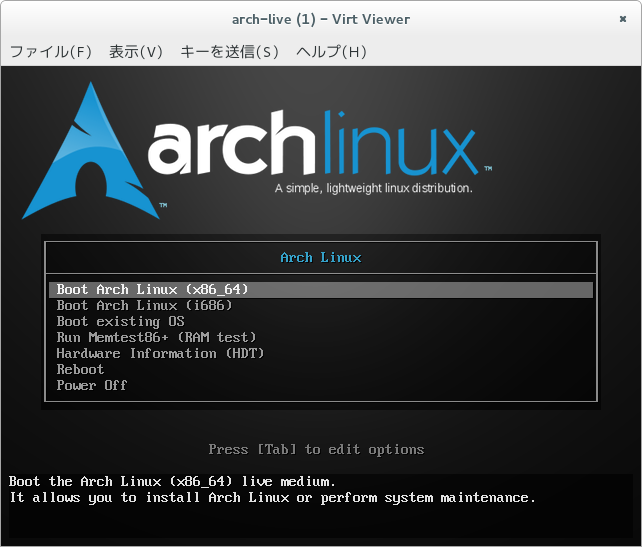
\includegraphics[width=0.7\hsize]{image201411/arch-boot.png}
\end{center}
\caption{Arch Linux isoイメージブートの様子}
\end{figure}
\end{frame}

\begin{frame}{Arch LinuxをKVMにインストール}

  詳しい手順は、第 120 回 東京エリア Debian 勉強会資料を参照。\\
  \url{http://tokyodebian.alioth.debian.org/pdf/ debianmeetingresume201411.pdf}\\

  基本的に、インストーラが無いので、手動でインストールとなります。
\end{frame}

\begin{frame}{Debianとの違い}

  第 120 回 東京エリア Debian 勉強会資料の表1を参照。\\
  \url{http://tokyodebian.alioth.debian.org/pdf/ debianmeetingresume201411.pdf}\\

\end{frame}

\begin{frame}{Arch Linuxを図示}
\begin{figure}[H]
\begin{center}
 \includegraphics[width=0.9\hsize]{image201411/arch-schema.eps}
\end{center}
\caption{Arch Linux}
\end{figure}
\end{frame}

\begin{frame}{参考:Debianを図示}
\begin{figure}[H]
\begin{center}
 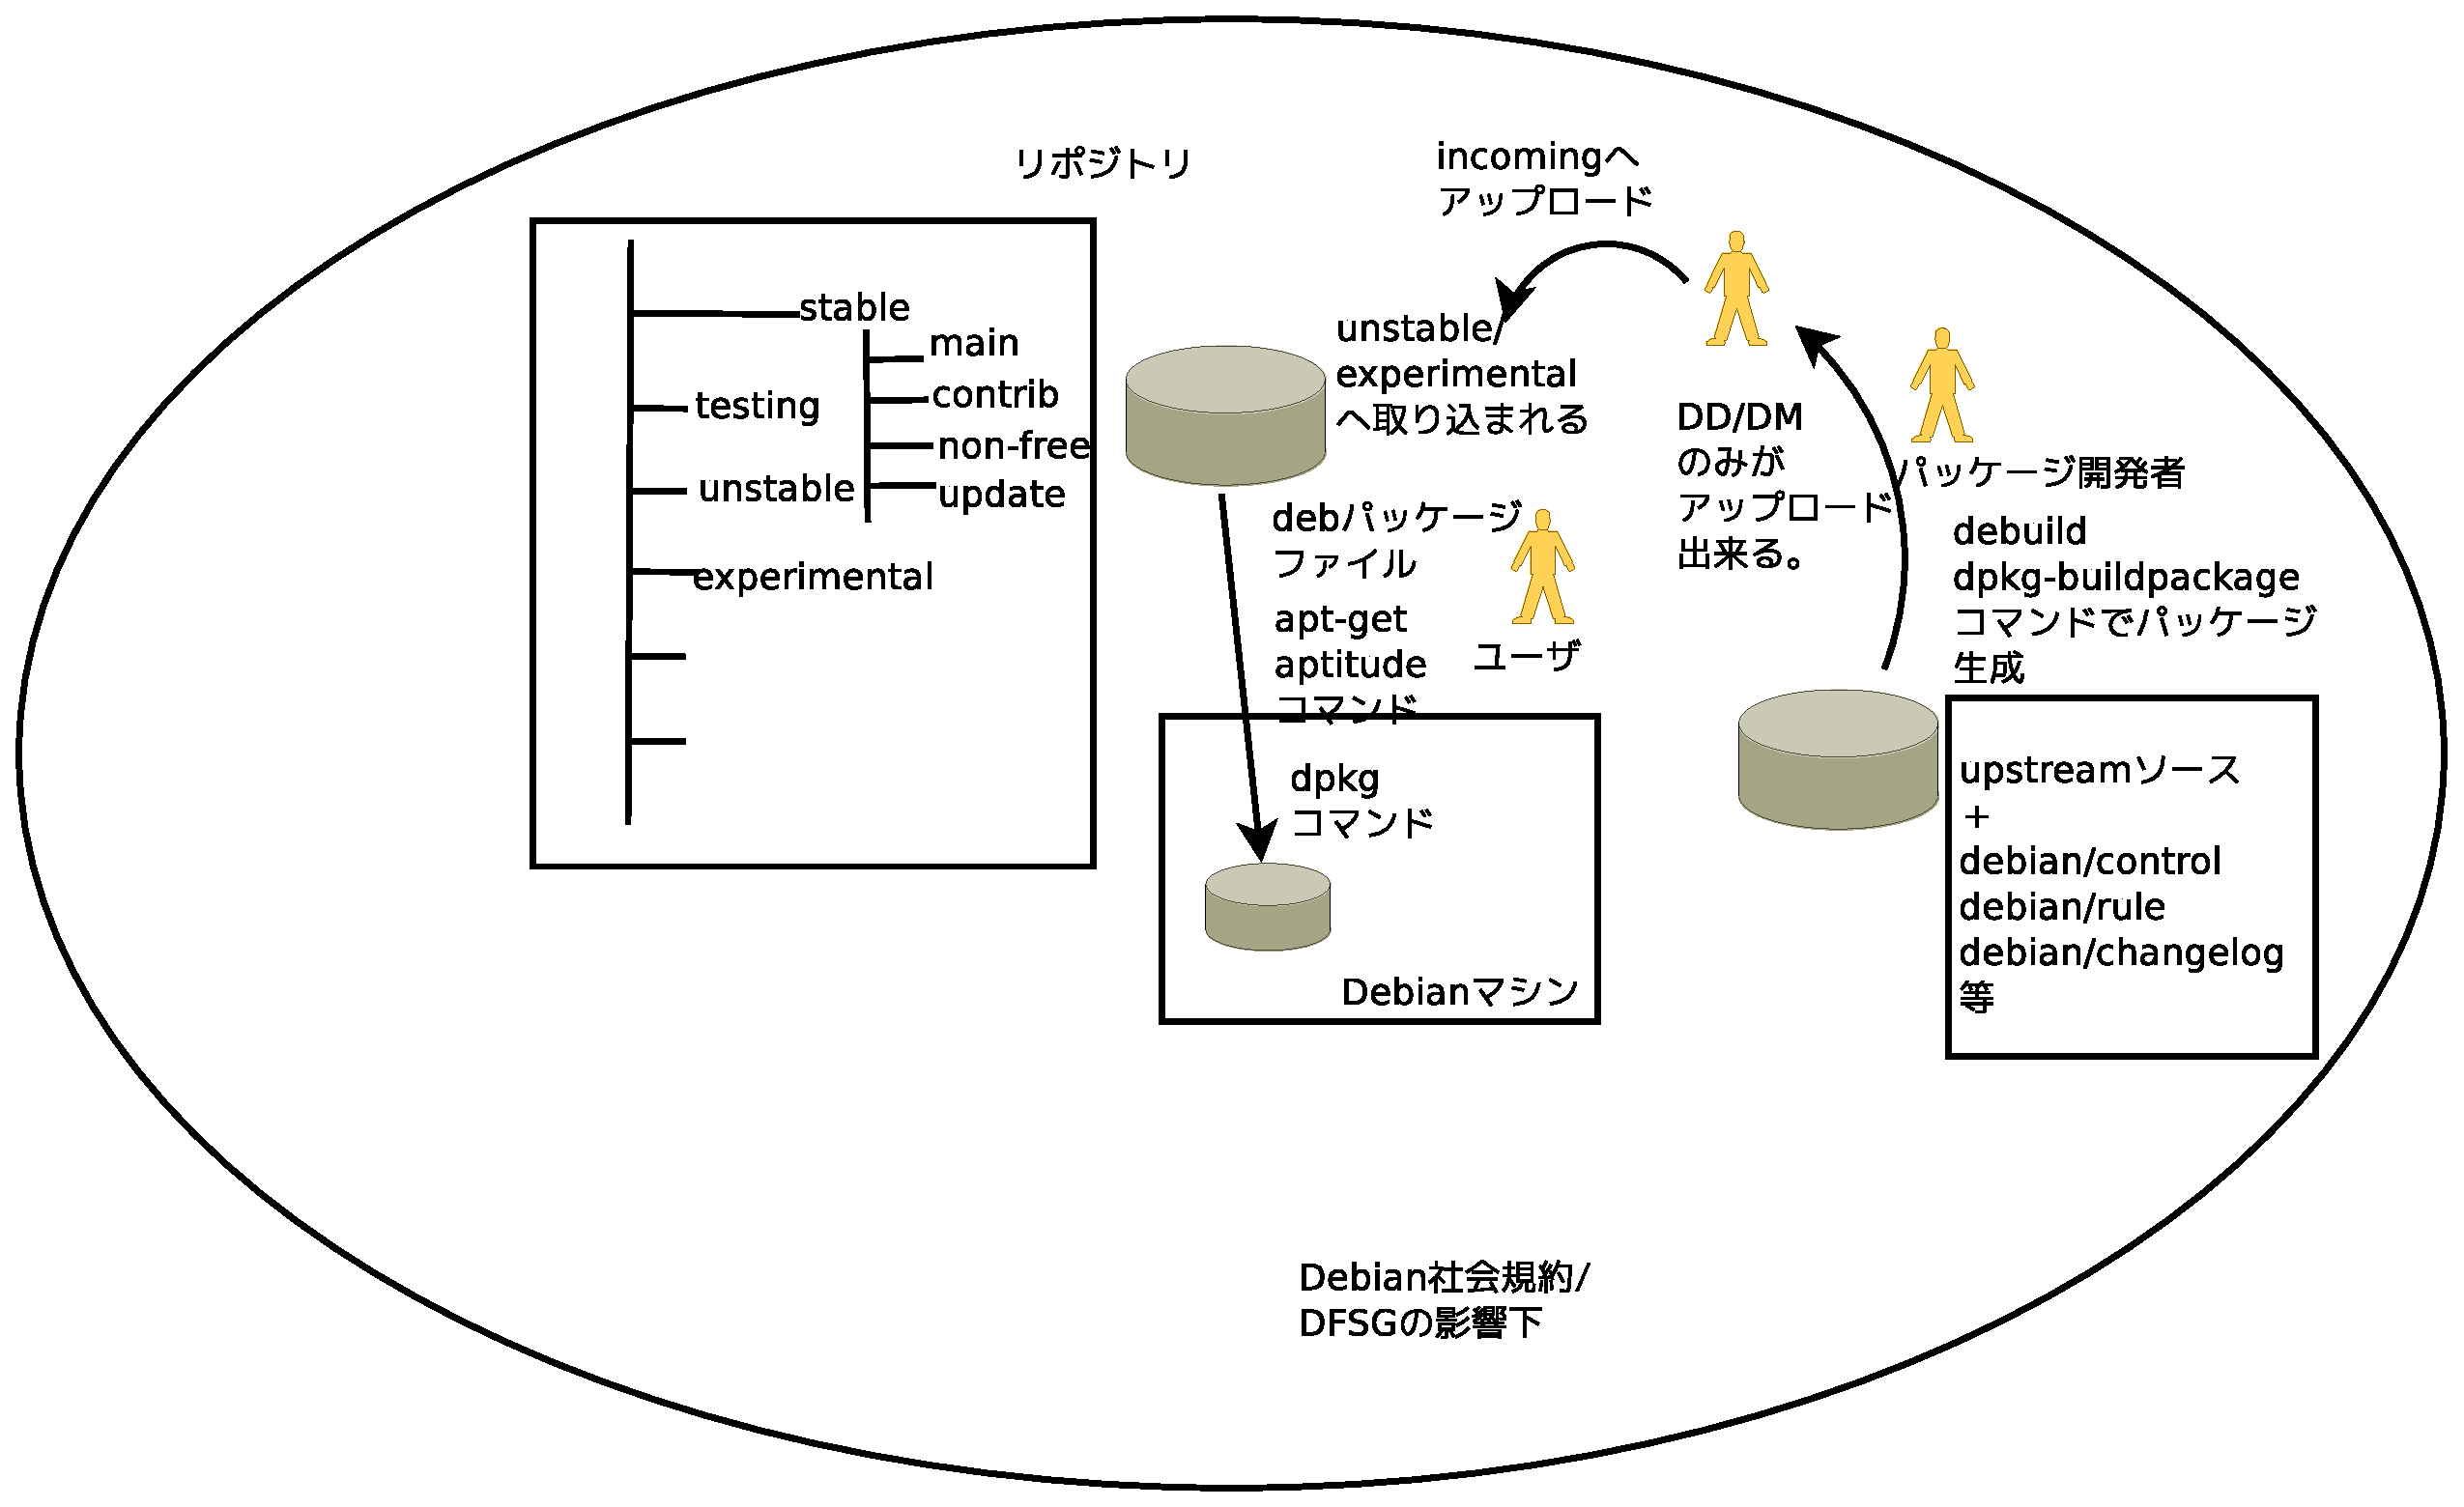
\includegraphics[width=0.9\hsize]{image201411/debian-schema.eps}
\end{center}
\caption{参考:Debian}
\end{figure}
\end{frame}

\begin{frame}{AUR}
\begin{itemize}
\item Arch Linuxには、officialリポジトリに含まれないソフトウェアについて、ユーザがPKGFILE等のbuildファイル一式をアップロードして他のユーザと共有して使う為に使うリポジトリ
\item AURから入手できるyaourt(ヨーグルトと読む)コマンドを使うと、AURをあたかもpacmanで扱ったかのように便利に使える。
\item  AURに登録されたbuildファイルはユーザの投票により、一定量の支持が得られると、Trusted User(TU)らにより、officialリポジトリのcommunityリポジトリに取り込まれる仕組みのようです。
\end{itemize}
\end{frame}

\begin{frame}{AUR注意点}

   登録されたbuildファイルは誰も精査していない場合があるため、基本的には自己責任(AT YOUR OWN RISK)での活用が基本です。

\end{frame}  

\begin{frame}{Arch Linuxの良さ}
\begin{itemize}
\item The Arch Wayに記載されているとおり、Arch Linuxを構成するあらゆるソフトウェアは最小限主義に貫かれています。従って、upstreamのソフトウェアとの変更点も最小としている為、設定ファイルの見通しが非常に良いです。
\item ユーザフレンドリということには重おきをおかず、ユーザの嗜好を極力邪魔しない(User Centerized)事をモットーとしているため、ユーザ自身が欲しいソフトウェアだけを導入という事がやりやすい作りになっています。
\end{itemize}

\end{frame}

\begin{frame}{Arch Linuxの良さ(つづき)}
\begin{itemize}
\item AURのように、利用者が自由にbuildファイルを登録できる仕組みがあるため、気軽にパッケージを公開することが出来ます。また、upstreamとの変更点を最小限に保つ方針のため、パッケージ化にかかる労力が少なくて済み、upstream側のリリースにあわせてスピーディーにパッケージ側のバージョンを追従させるが可能です。
\item 軽量です。パッケージを厳選して導入する事がしやすいため、マシンのスペックが低くても問題になりにくいです。
\end{itemize}
\end{frame}

\begin{frame}{終わりに}

結論:
\begin{itemize}
  \item Arch Linuxはシンプルかつ最小限をモットーとしており、ソフトウェアの個別設定を自力で行う必要があります。そのため、Linuxシステムの勉強を熱心にしたい人、あるいは、導入するソフトウェアに強いこだわりがある人は、うってつけのシステムかと思います。
 \item Debianは最初からある程度便利に使えるようにいろいろと自動で設定が行われ、マシン資源を消費するものの多くの便利なパッケージをある程度の量勝手に導入しておいてくれることを期待する人向けかと思います。
\end{itemize}
\end{frame}

\begin{frame}{結局のところ}

 Debianの良い所を正確に知る、あるいは目指すべき方向性の確認には、他のディストリビューションと比較することも重要かと思います。機会があれば、他のディストリビューションも使ってみて、Debianとの比較を行うのもよいのではないでしょうか。

\end{frame}

\section{今後のイベント}
\emtext{今後のイベント}
\begin{frame}{今後のイベント}
\begin{itemize}
 \item 関西エリアDebian勉強会
 \item 東京エリアDebian勉強会 
\end{itemize}
\end{frame}

\section{今日の宴会場所}
\emtext{今日の宴会場所}
\begin{frame}{今日の宴会場所}
未定
\end{frame}

\end{document}

;;; Local Variables: ***
;;; outline-regexp: "\\([ 	]*\\\\\\(documentstyle\\|documentclass\\|emtext\\|section\\|begin{frame}\\)\\*?[ 	]*[[{]\\|[]+\\)" ***
;;; End: ***
